\documentclass[12pt]{article}
\title{Expense CLI: A Command-Line Expense Management Program}
\author{Kyle Dormer (S1802423)}
\date{January 13, 2019}
\usepackage{graphicx}
\usepackage{listings}
\usepackage{hyperref}
\usepackage{float}


\begin{document}
  \pagenumbering{gobble}
  \maketitle
  \tableofcontents
  \newpage
  \pagenumbering{arabic}

  \section{Introduction}
  This piece of software is a command-line expense management tool. Its intended purpose is to allow the user to enter their income and their expenses and to have them stored and tracked for them. More specifically, the objectives of the software are that the user should be able to:
  \begin{itemize}
    \item Enter their monthly income, be it from single or from multiple sources.
    \item Set an overall monthly budget as well as a budget for categories of expense.
    \item Enter their expenses based on expense categories.
    \item Add new expense categories.
    \item View an exense report in terms of day/week/month/year and also with respect to a category.
    \item Generate and export a graph of their expenses in \textit{PDF} format.
    \item The expense report should should inform the user when they are over/under budget for a specific category in a specific month.
    \item The expense report should also display the average expense per category.
    \item These objectives should be achieved using a backend \textit{SQLite} database and with the \textit{Pandas} and \textit{Matplotlib} modules.
  \end{itemize}
  In retrospect to the development process, all of these objectives have been successfully implemented and achieved relatively smoothly and without issue. The biggest problems faced throughout the development of the software involved averaging the expenses of the user while generating the expense report. Furthermore, displaying the user's expenses in a nicely formatted fashion in a command-line environment proved difficult, as opposed to implementing a \textit{GUI} solution. The format was solved by designing an algorithm that makes use of Python's concept of \textit{list comprehension} in synergy with the inbuilt \textit{any()} function.
  \section{Design of System}
  \subsection{Design Paradigm}
  First and foremost, the design of the software is based upon the \textit{procedural} programming paradigm, derived from the \textit{imperative} paradigm.
  This can very much be reflected in the structure of the codebase. The program functions by the \textit{\_\_main\_\_} module making a call to the \textit{main()} function or \textit{procedure}, which in turn make calls to other functions which also make calls to other functions. An example of this can be observed within \textit{expcli.py}.
    \begin{lstlisting}[language=Python, caption=An example of procedural program design from \textit{expcli.py}, captionpos=b]
    option_choice = get_user_option([])

    if option_choice[0] == 1:
        get_income()

    elif option_choice[0] == 2:
        monthly_budget = get_monthly_budget([])
        sql.store_monthly_budget(monthly_budget[0])

    elif option_choice[0] == 3:
        expense = get_expense()
        sql.store_expense(expense)

    elif option_choice[0] == 4:
        categories = get_categories([])
        sql.store_categories(categories)

    elif option_choice[0] == 5:
        date = get_expense_date([])
        expenses = get_display_expenses('day', date[0], None)
        display_expenses(expenses)
    \end{lstlisting}
  As shown in Listing 1, the program obtains the user's choice for which option to take. Depending on the user's choice, the \textit{control flow} of the program is determined by making a function call to the function that corresponds with the user's choice. In fact, when combined with \textit{recursion}, this is how the entirety of the program functions; the user enters their option, the corresponding function calls are made, and then the user enters another option \textit{ad infinitum}.

  The procedural paradigm was chosen in the design of this program due to its focus on using \textit{variables}, \textit{data structures} and \textit{functions} to design and carry out algorithmic tasks. Whereas, for example, the \textit{object-oriented} design paradigm focuses on conceptualising real world concepts as objects that contain both data and methods to interact with said data. In the context of this program, user expenses and input are stored as data structures, more specifically as lists of dictionaries. Therefore, using procedurally designed functions to interact with this data makes more sense. Furthermore, object-oriented programing is often less efficient than procedural programming\cite{luca}, and with the relatively simple nature of the data involved in this program (expenses have only 4 properties), object-oriented was not deemed necessary nor favourable. 

  \subsection{Modular Programming}
  In combination with the procedural paradigm, the technique of \textit{modular programing} has also been focused upon throughout the design of this program.
  There are multiple reasons for this design choice. 

  Firstly, splitting the program into individual modules that each handle one area of functionality effectively \textit{encapsulates} complexity. Therefore, once a module has been implemented and thoroughly tested, it can be reused by I or another programmer without knowing how it works. All the knowledge required to use it would be its purpose, its arguments (if it has any) and its output.
  An example of this can be observed many times throughout the codebase of the program, although most notably in the usage of the \textit{exptools} module.
  \begin{lstlisting}[language=Python, caption=An example of encapsulation achieved via modular programming in \textit{expcli.py}, captionpos=b]
    def get_monthly_budget(budget_var):

      monthly_budget = input('Enter monthly budget: ')

      if ex.validate_input(monthly_budget, 1, 18, str):
          try:
              monthly_budget = float(monthly_budget)
              budget_var.append(monthly_budget)

          except (Exception):
              ex.print_important('Invalid number, please try again!')
              get_monthly_budget(budget_var)
      else:
          ex.print_important('Invalid number, please try again!')
          get_monthly_budget(budget_var)

      return budget_var
    \end{lstlisting} 

  This function's purpose is to recursively collect a monthly budget from the user and makes use of the \textit{validate\_input()} and \textit{print\_important()} functions from the \textit{exptools} module, although in this context its module object is defined as \textit{ex} for shorthand use.

  Secondly, as alluded to in the first point, modular programming allows for very effective \textit{code reuse}. Indeed, this was in fact the original reasoning behind the creation of modular programming, first implemented in \textit{ALGOL 68-R} in 1970.\cite{algol}. As can be seen in Listing 2, the \textit{validate\_input()} function can be called (reused) whenever needed.

  Thirdly and finally, modular programming achieves \textit{separation of concerns}. This means that each concern (or aspect of functionality) of the program belongs to a self-contained module. This ties in with the first point in that it allows the code of modules to change completely and still work perfectly as long as their expected inputs and outputs remain the same to interface properly with the rest of the program.
  \subsection{Recursion}
  Most of the functions, especially functions that gather user input, in this program shall be \textit{recursive}. This involves a function calling itself to achieve a purpose. This is very useful in obtaining user input which must be validated for length or type. One objective of the program is to allow the user to enter their expenses. This will involve the expense's category, expense's date and the expense's amount; a string, string (or \textit{datetime} object) and a float respectively. Furthermore, the strings must be between a minimum and maximum length. However, it is unlikely that the user will perfectly enter the desired input in a proper fashion each time. Therefore if validation of the user's input fails, the program should alert the user to the correct format of input and prompt them again.
  An algorithm for this could be implemented as pseudocode as such.
    \begin{lstlisting}[caption=An example pseudocode algorithm to inefficiently obtain valid user input, captionpos=b]
      WHILE TRUE:
        GET input
        IF VALIDATE input FALSE:
          GET input
    \end{lstlisting}

  However, this algorithm is flawed in that the user may not enter the input in the correct format even after being prompted, and to deal with this the \textit{if} block would have to keep nesting under itself \textit{ad infinitum}.
  Therefore, instead of having an infinite loop and a potentially infinite control structure, the function could simply call itself again if the user does not enter the input correctly. This would be resource efficient as it would only be called as much as needed and would simplify and reduce the lines of code needed to be written.
  The pseudocode for this newly imagined algorithm can be expressed in Listing 4.
    \begin{lstlisting}[caption=A correct\, recursive algorithm to obtain valid user input, captionpos=b]
      SUB get_input:
        GET input
        IF VALIDATE input TRUE:
          RETURN input
        ELSE:
          get_input
    \end{lstlisting}

    An implementation of the Listing 4 algorithm can be observed in Listing 2.
    This algorithm will be repurposed throughout the program for whenever the user needs to input data (expenses, expense categories, income sources, and monthly budget).

  \subsection{Algorithms for the Objectives}
  The purpose of this section is to specify algorithms that achieve each objective set out in the specification.
  \subsubsection{Control Flow}
  The overall algorithm has been alluded to previously. It will display the options to the user and procedurally carry out the desired option and then recursively allow the user to enter another option (unless the user opts to exit the program).

  The flowchart for this algorithm can be expressed as such.
  \begin{figure}[H]
    \centering
    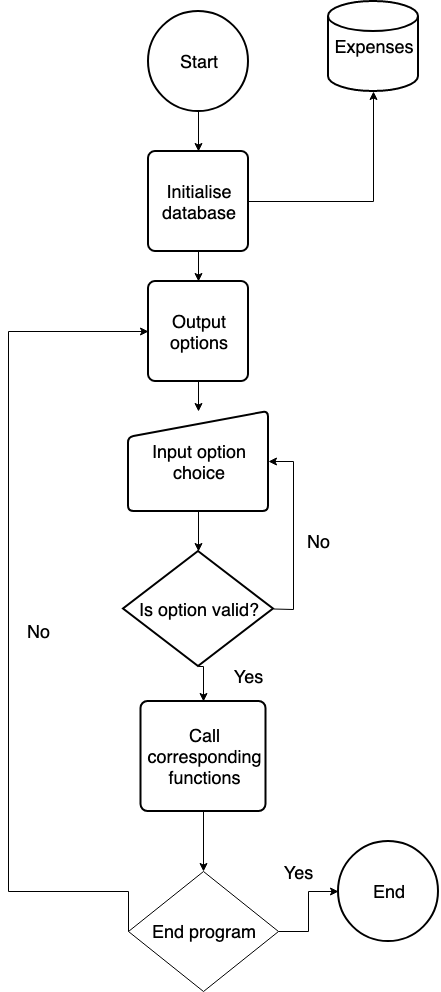
\includegraphics[scale=0.4]{overall_program_flow.png}
    \caption{The overall control and execution flow of the program.}
  \end{figure}
  


  \section{Testing the System}
  \section{Demonstrating the System}

  \appendix
  \section{User Guide}
  \section{Code}
  \section{Test Suites}

  \begin{thebibliography}{9}
    \bibitem{luca}
    Cardelli, Luca (1996),
    \textit{Bad Engineering Properties of Object-Oriented Languages},
    Digital Equipment Corporation Systems Research Center
    Sourced from: \url{http://lucacardelli.name/Papers/BadPropertiesOfOO.html},
    Accessed: [22nd January 2020].

    \bibitem{algol}
    C. H. Lindsey (University of Manchester) \&
    H. J. Boom (Mathematisch Centrum, Amsterdam),
    \textit{A Modules and Separate Compilation Facility for ALGOL 68},
    Sourced from: \url{http://archive.computerhistory.org/resources/text/algol/ACM_Algol_bulletin/1061719/p19-lindsey.pdf},
    Accessed: [22nd January 2020].


  \end{thebibliography}

\end{document}
